

% Definitionen



%%%%%%%%%% Kopfbereich %%%%%%%%%%%%%
%\documentclass[a4paper,titlepage,oneside,fontsize=2pt]{scrbook} % Dokumentklasse
\documentclass[11pt,a4paper,titlepage,oneside]{report} % Dokumentklasse
\usepackage{titlesec}



\titleformat{\chapter}[display]
{\normalfont\huge\bfseries}{\chaptertitlename\ \thechapter}{20pt}{\Huge}
\titleformat{\section}
{\normalfont\Large\bfseries}{\thesection}{1em}{}
\titleformat{\subsection}
{\normalfont\large\bfseries}{\thesubsection}{1em}{}
\titleformat{\subsubsection}
{\normalfont\normalsize\bfseries}{\thesubsubsection}{1em}{}
\titleformat{\paragraph}[runin]
{\normalfont\normalsize\bfseries}{\theparagraph}{1em}{}
\titleformat{\subparagraph}[runin]
{\normalfont\normalsize\bfseries}{\thesubparagraph}{1em}{}

\titlespacing*{\chapter} {0pt}{-50pt}{20pt}
\titlespacing*{\section} {0pt}{3.5ex plus 1ex minus .2ex}{2.3ex plus .2ex}
\titlespacing*{\subsection} {0pt}{3.25ex plus 1ex minus .2ex}{1.5ex plus .2ex}
\titlespacing*{\subsubsection}{0pt}{3.25ex plus 1ex minus .2ex}{1.5ex plus .2ex}
\titlespacing*{\paragraph} {0pt}{3.25ex plus 1ex minus .2ex}{1em}
\titlespacing*{\subparagraph} {\parindent}{3.25ex plus 1ex minus .2ex}{1em}



\pdfminorversion=7  %akzeptiert pdf in version 1.7
%\RequirePackage{pdf14}
\usepackage{etex}
\usepackage[ansinew]{inputenc}

\usepackage{lipsum}

\usepackage{nomencl,longtable,ifthen} % Symbolverzeichnis
%\usepackage{ngerman} % Deutsch, neue Rechtschreibung
%\usepackage[latin1]{inputenc} % Sonderzeichen ��� etc.
\usepackage[T1]{fontenc} % T1 Format
\usepackage{geometry} % Seitenr�nder
\usepackage[printonlyused]{acronym} % Abk�rzungsverzeichnis
\usepackage{graphicx} % Einbinden von Grafiken
\usepackage{fancyhdr} % Gestaltung von Kopf- und Fu�zeile
%\usepackage{bibgerm} % Literaturverzeichnis
%\usepackage[squaren]{SIunits} % SI Einheiten
\usepackage{amsmath, amsthm, amssymb}
\usepackage{mathtools}
\usepackage{floatflt}
\usepackage{float}
\usepackage{graphics}
%\usepackage{picins}
\usepackage{wrapfig}
\usepackage{threeparttable}
\usepackage{textcomp}
\usepackage{tabularx}
\usepackage{hhline}
\usepackage{siunitx}
\usepackage{framed, color}

\usepackage{courier}
\usepackage{listings}
\usepackage{color}
\usepackage{multicol}
\usepackage{multirow}
\usepackage[hyphens]{url}
\usepackage{xcolor}
\usepackage[right]{eurosym}
\usepackage{colortbl}
\usepackage{subfigure}
\usepackage{setspace}
\usepackage{footnote}
\usepackage{wasysym}
% Seitenstil definieren
\pagestyle{fancy}
\fancyhead{}
\fancyfoot{}
\rhead{\leftmark}
\cfoot{\thepage}
\renewcommand{\headrulewidth}{0pt}
\renewcommand{\footrulewidth}{0.4pt}

\usepackage[bottom]{footmisc}
%\usepackage{footmisc}
\setlength{\footnotemargin}{2mm} % Einr�cken der Fu�note
\setlength{\footnotesep}{12pt}% Abstand zwischen den Fu�noten 
\setlength{\skip\footins}{22pt}% Abstand Zwischen Haupttext und Fu�noten

%-------------------------------
\usepackage{calc}

% Paket f�r Zeichnungen
\usepackage{tikz}
\usepackage{tikz-timing}
\usepackage{vhistory}
%

\usetikztiminglibrary[new={char=Q,reset char=R}]{counters}
\usetikztiminglibrary{arrows}
\usetikzlibrary{shapes,
								arrows,
								calc,
								automata,
								positioning,
								mindmap,
								fit,
								trees,
								shadows,
								decorations,
								scopes,
								matrix,
								chains,
								shapes.misc,% wg. rounded rectangle
  							shapes.arrows,%
  							decorations.pathmorphing}



%-------------------------------
\usepackage[plainpages=false]{hyperref}
\hypersetup{colorlinks%Rot im inhaltsverzeichniss entfernt"'
,linkcolor=black
,filecolor=blue
,urlcolor=blue
,citecolor=blue}

%\pdfoptionpdfminorversion=6
%\pdfminorversion=7  %akzeptiert pdf in version 1.7
\setcounter{tocdepth}{3} %%f�r subsubsection!!!
\setcounter{secnumdepth}{3} 
%\usepackage{watermark}
\definecolor{light}{gray}{.50}



%%%%%%%%% Neue Kommandos %%%%%%%%%%%%%
\let\abk\nomenclature % Abk�rzung shortcut
\newcommand{
\changefont}[3]{\fontfamily{#1} \fontseries{#2} \fontshape{#3} \selectfont} % Setzen der Schriftart



%%%%%%%%%%%%%% zus�tzliche unit-Spalte %%%%%%%%%%%%%%%%
\newcommand{\nomunit}[1]{%
\renewcommand{\nomentryend}{\hspace{2em}\hspace*{\fill}#1}}


%%%%%%%%%%%%%% longtable an Stelle der Liste %%%%%%%%%%
\makeatletter
\def\@@@nomenclature[#1]#2#3{%
   \def\@tempa{#2}\def\@tempb{#3}%
   \protected@write\@nomenclaturefile{}%
      {\string\nomenclatureentry{#1\nom@verb\@tempa @{\nom@verb\@tempa}&%
         \begingroup\nom@verb\@tempb\protect\nomeqref{\theequation}%
            |nompageref}{\thepage}}%
   \endgroup
   \@esphack}
\def\thenomenclature{%
   \@ifundefined{chapter}{\section*}{\chapter*}{\nomname}%
   \nompreamble
   \begin{longtable}[l]{@{}ll@{}}}
\def\endthenomenclature{%
\end{longtable}
\nompostamble}
\makeatother


%%% Listings
\definecolor{LinkColor}{rgb}{0,0,0.5}
\definecolor{ListingBackground}{rgb}{0.9,0.9,0.9}
\definecolor{dunkelgrau}{rgb}{0.8,0.8,0.8}
\definecolor{lightblue}{rgb}{0.6132,0.7382,0.8554}
\definecolor{lightwhite}{rgb}{1,1,1}
\definecolor{schwarz}{rgb}{0,0,0}
\definecolor{weiss}{rgb}{1,1,1}
\definecolor{codegreen}{rgb}{0,0.5,0}
\definecolor{codegray}{rgb}{0.0,0.5,0.5}
\definecolor{codepurple}{rgb}{0.5,0,0.5}
\definecolor{backcolour}{rgb}{0.95,0.95,0.92}


\lstloadlanguages{C} % TeX sprache laden, notwendig wegen option 'savemem'
\lstset{%
	language=C,     				% Sprache des Quellcodes ist TeX
commentstyle=\color{codegreen},
    keywordstyle=\color{blue}\bfseries,
    numberstyle=\tiny\color{codegray},
    stringstyle=\color{codepurple},
	numbers=left,            % Zelennummern links
	stepnumber=1,            % Jede Zeile nummerieren.
	numbersep=5pt,           % 5pt Abstand zum Quellcode
	numberstyle=\tiny,       % Zeichengr�sse 'tiny' f�r die Nummern.
	breaklines=true,         % Zeilen umbrechen wenn notwendig.
	breakautoindent=true,    % Nach dem Zeilenumbruch Zeile einr�cken.
	postbreak=\space,        % Bei Leerzeichen umbrechen.
	tabsize=2,               % Tabulatorgr�sse 2
	basicstyle=\ttfamily\footnotesize, % Nichtproportionale Schrift, klein f�r den Quellcode
	showspaces=false,        % Leerzeichen nicht anzeigen.
	showstringspaces=false,  % Leerzeichen auch in Strings ('') nicht anzeigen.
	extendedchars=true,      % Alle Zeichen vom Latin1 Zeichensatz anzeigen.
	captionpos=b, %Caption unten
	backgroundcolor=\color{weiss}} % Hintergrundfarbe des Quellcodes setzen.


%%%%%%%%%%%%%%%%%%%%%%%%%%%%%%%%%%%%%%%%%%

\lstdefinelanguage{Assembler}%
   {morekeywords={BL,LDR,MOV,bx,sub,stmfd,ldr,str,mrs,msr,ldmia},%
    morekeywords=[2]{.global,.extern,.macro,.endm},%
    alsoletter={.,0,1,2,3,4,5,6,7,8,9},%
    alsodigit={?},%
    sensitive=false,%
    morestring=[b]",%
    morecomment=[s]{/*}{*/},%
    morecomment=[l]@,%
    morecomment=[l]//,%
   }[keywords,comments,strings]

%%%%%%%%% Erstellung der Verzeichnisse %%%%%%%%%%%%%
\makenomenclature
%\makeglossaries
%\makeindex

%%%%%%%%% Seitenlayout %%%%%%%%%%%%%
\setlength{\parindent}{0pt} % Zeileneinzug bei Absatz
\linespread{1.3} % hor. Zeilenabstand
%\geometry{a4paper, top=40mm, left=35mm, right=25mm, bottom=40mm, headsep=10mm, footskip=10mm} % Randabst�nde kl�ren

\geometry{a4paper, top=40mm, left=30mm, right=30mm, bottom=40mm, headsep=10mm, footskip=10mm} % Randabst�nde kl�ren
\setlength{\headheight}{5pt}

\usepackage{tabu}

\usepackage{booktabs}% http://ctan.org/pkg/booktabs
\newcommand{\tabitem}{~~\llap{\textbullet}~~} % Include Packages

% to fix grouping in the list of .......
\let\Chapter\chapter
\def\chapter{\addtocontents{lol}{\protect\addvspace{10pt}}\Chapter}

%%%%%%%%% Dokumentenbeginn %%%%%%%%%%%%%%%
\begin{document}


\title{TITLE}
\author{NAME}

%\nomenclature[gz]{}{\nomunit{}}
%\changefont{cmr}{m}{n},
%\fontsize{12}{15}
%\selectfont


%Titelseite
\pagenumbering{Alph}

% %%%%%%% Titelseite %%%%%%%%%%%%%
\begin{titlepage}
\newgeometry{top=20mm, left=20mm, right=20mm, bottom=20mm}

\begin{center}
\begin{table}              
\begin{tabular}{ll}

\includegraphics[width=6cm]{images/logo_hse.jpg} 
\end{tabular}
\end{table}
\end{center}

\begin{center}\huge
\vspace*{2mm}
\textbf{Work Package}\\

\vspace{17mm}

%\raggedright
\textsc{Server Administration itlx3304 and itlx3301
} \\
\textsc{Version 2.0
}

\end{center}


\newpage

\topskip0pt
\vspace*{\fill}

\begin{center}

\vspace{17mm}

\singlespacing
\textbf{\huge{Vikas Agrawal}}

\vspace{5mm}

\large{\textsc{Hochschule Esslingen}}\\
\large{{Faculty of Computer Science}}\\

\vspace{5mm}
%\begin{tabbing}
\large{Supervisor:  Prof. Joerg Friedrich}\\
%\end{tabbing}

\vspace{5mm}
\large{\today}\\

\vspace*{\fill}

\end{center}

\end{titlepage}
 % Erkl�rung
\restoregeometry % Manipulierte Seitenr�nder wiederherstellen.
\setcounter{page}{2}
%\chapter*{}
\thispagestyle{empty}  % Leerseite mit Alpha Buchstaben


%%%%%%%%%% Externe Seiten %%%%%%%%%%%%%
%
%%%%%%%%%% Verzeichnisse, Erkl�rungen etc. %%%%%%%%%%%%%
%{
\pagestyle{plain} % Leere Seiten
%\include{parts/blankpage} % Leerseite
\pagenumbering{Roman} % R�mische Seitennummerierung f�r die ersten Seiten


%\include{parts/Sperrvermerk} % Sperrvermerk
%\include{parts/Erklaerung} % Erkl�rung
%\include{parts/Abstract} % Kurzfassung

%------------------
%Versioning page
%\begin{document}
% Start of the revision history table
\begin{versionhistory}
  \vhEntry{1.0}{22 August, 2015}{Vikas Agrawal}{created}
  \vhEntry{2.0}{7 September, 2015}{Vikas Agrawal}{sent to Friedrich}
  \vhEntry{2.0}{12 December, 2015}{Vikas Agrawal}{adding itlx3304}
\end{versionhistory}
\pagebreak
%------------------

\pdfbookmark[1]{Table of contents}{toc} % PDF-Bookmark f�r Inhaltsverzeichnis setzen
\tableofcontents % Inhaltsverzeichnis
\clearpage

%
\phantomsection
\addcontentsline{toc}{chapter}{Abbreviations}
\chapter*{List of Abbreviations} % Kapitel Abk�rzungsverzeichnis (ohne Nummerierung)
\markboth{List of Abbreviations}{List of Abbreviations}

\begin{acronym}[XXXXXXXXX]
%\renewcommand{\bflabel}[1]{\normalfont{\normalsize{#1}}\hfill}  %Serivenschrift
\setlength{\itemsep}{-\parsep}
	
%\singlespacing
  \acro{Abbreviation}{Description}
  \vspace{6mm}%\acro{}{}
	\acro{RTC}{Real Time Clock}

	%-----------------
	
\onehalfspacing
\end{acronym}
\addcontentsline{toc}{section}{List of Abbreviations}	% in Inhaltsverzeichnis aufnehmen



%\clearpage

%\include{parts/Symbolverzeichniss}
%\clearpage
%------------------------
%------------------------

\pagenumbering{arabic} % Arabische Seitennummerierung f�r den Hauptteil
\onehalfspacing

% Kapitelanfangsseiten umgestalten
\fancypagestyle{plain}{
\fancyhf{}
\cfoot{\thepage}\renewcommand{\headrulewidth}{0pt}} 


%%%%%%%%% Hauptteil %%%%%%%%%%%%%
\pagestyle{fancy}
%\include{parts/Einleitung}
	
\chapter{Setting itlx3304}


\begin{itemize}
 \item Apache configuration
 \subitem wwwitrt.conf
 \subitem dav\_svn.conf
 \subitem jk.conf
 \subitem shibboleth.conf
 \item LDAP configuration
 \item Jenkins configuration
 \item SVN configuration
 \item Trackplus configuration
 \item MySql configuration
 \item PWM configuration
\end{itemize}

\section{Trackplus Configuration}
To integrate Jenkins and other web applications in trackplus, we need to
download portal$5.0$ from the trackplus website. This plugin has to be
configured and urls of the webapplications needs to be written in the
configuration file inside the portal$5.0$ directory.
The plugin to be downloaded from the trackplus website has the extension .tpx.
 
\section{MySql configuration}
MySql is a database and needs to be configured for trackplus. First of all a
database is created, but for that one needs to know the root password of MySql.
The root password is kept under the folder called /root in the server.
mysql -uroot -ptissi
mysql -utrackp -ptissi
mysql -uroot -p (password in the /root folder)


\chapter{Removing legacy code from SVN}
\section{Deleting and
moving old SVN Repositories in itlx3301}As of August, $22015$, there were seven
SVN repositories excluding lab team repositories\\\\
\begin{figure}[H]
\begin{center}
		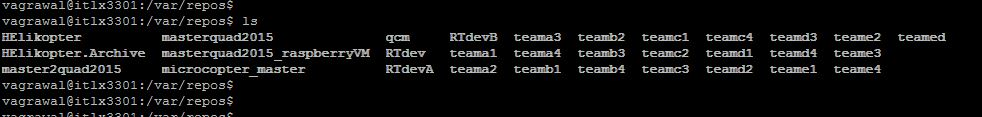
\includegraphics[width=1.0\textwidth]{images/svn_repos_before.jpg} 
		\caption{Repos before changes}
	\label{fig:SVNBefore}
\end{center}
\end{figure}

\begin{enumerate}
  \item HElikopter
  \item HElikopter.Archive
  \item microcopter\_master
  \item masterquad$2015$
  \item masterquad$2015$\_raspberryVM
  \item master$2$quad$2015$
  \item DOSEK
\end{enumerate}

\section{Moving the repositories}
\begin{itemize} 
  \item
  \textbf{HElikopter}
  \url{svn+ssh://vagrawal@itlx3301.hs-esslingen.de/var/repos/HElikopter/trunk} This is the HElikopter source code on the code warrior and is maintaned by Hr.
  Trybek. The underlying microcontroller is the dragon board running the
  Freescale microcontroller. The project has the milestone REL$210$ as of
  $01.10.2014$.
  The repositories HElikopter is merged into git repoitories kept at
  \url{https://atreus.informatik.uni-tuebingen.de/agrawal/helikopter-software}.
  However the svn repository still exists since Hr Trybek works on the
  repository.
  
  \item
  \textbf{HElikopter.Archive}
  \url{svn+ssh://vagrawal@itlx3301.hs-esslingen.de/var/repos/HElikopter.Archive} This is a legacy project and has two tags REL$100$ from
  $24.04.2012$ and REL$200$ from $25.03.2013$.
  The SVN repository HElikopter.archive is moved to the
  Trash folder in /var/repos/. 
  The repositories HElikopteris merged into git repository kept at
  \url{https://atreus.informatik.uni-tuebingen.de/agrawal/helikopter-software},
  \item
  \textbf{microcopter\_master}
  \url{svn+ssh://vagrawal@itlx3301.hs-esslingen.de/var/repos/microcopter_master}
  The project also consists of the development of the HElikopter and consists of
  the matlab projects as well as the codewarrior projects. Last development in
  the project was in the year $2011$. This SVN repository has been moved to
  Trash under /var/repos and the contents has been merged in 
  \url{https://atreus.informatik.uni-tuebingen.de/agrawal/helikopter-simulation}
  and
  \url{https://atreus.informatik.uni-tuebingen.de/agrawal/helikopter-scratch}.
  \item
  \textbf{master2quad2015}
  \url{svn+ssh://vagrawal@itlx3301.hs-esslingen.de/var/repos/master2quad2015}
  This is a masters student $2015$ matlab project to make a matlab model of
  the HElikopter. This repository is deleted and the contents has been merged
  in the GIT repo \url{https://atreus.informatik.uni-tuebingen.de/agrawal/helikopter-simulation}
  \item
  \textbf{masterquad$2015$ and masterquad$2015$\_raspberryVM}
  \url{svn+ssh://vagrawal@itlx3301.hs-esslingen.de/var/repos/masterquad2015}
  This is a masters student $2015$ respberry project to make a raspberry based
  development of the HElikopter. The project consists of the ubuntu virtual
  machine which is a development environment and the source files consisting of
  the application and low lever drivers written for the raspberry.\\
  The repository masterquad$2015$ is moved to Trash under /var/repos and the
  content has been moved to two GIT Repositories.
  \url{https://atreus.informatik.uni-tuebingen.de/agrawal/helikopter-vm}
  and
  \url{https://atreus.informatik.uni-tuebingen.de/agrawal/helikopter-raspberry}.
  \item
  \textbf{LAB Team Repositores}
  The lab team project repositories are moved under the folder /var/repos/LABOR.
  \item
  \textbf{DOSEK}
  The DOSEK repositories are moved under the folder /var/repos/DOSEK.
  \end{itemize}
  
\section{SVN Repositories after changes}Now there are only two SVN
repositories excluding the lab team repositories\\
\begin{figure}[H]
\begin{center}
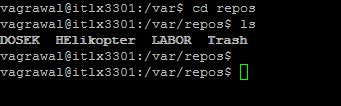
\includegraphics[width=1.0\textwidth]{images/svn_repos_after.jpg} 
\caption{Repos after changes}
\label{fig:SVNAfter}
\end{center}
\end{figure}
\begin{enumerate}
  \item HElikopter
  \item DOSEK
\end{enumerate}



\section{Exercises}
Team of Controller, Actuator and UI 
The students would study about the communication buses such as I2C, SPI, UART,
CAN.

\section{Slides}
\textbf{Estimation} : The process of inferring a value of a quantity of interest
from indirect, inaccurate and uncertain observations is called estimation.



\begin{figure}[H]
\begin{center}
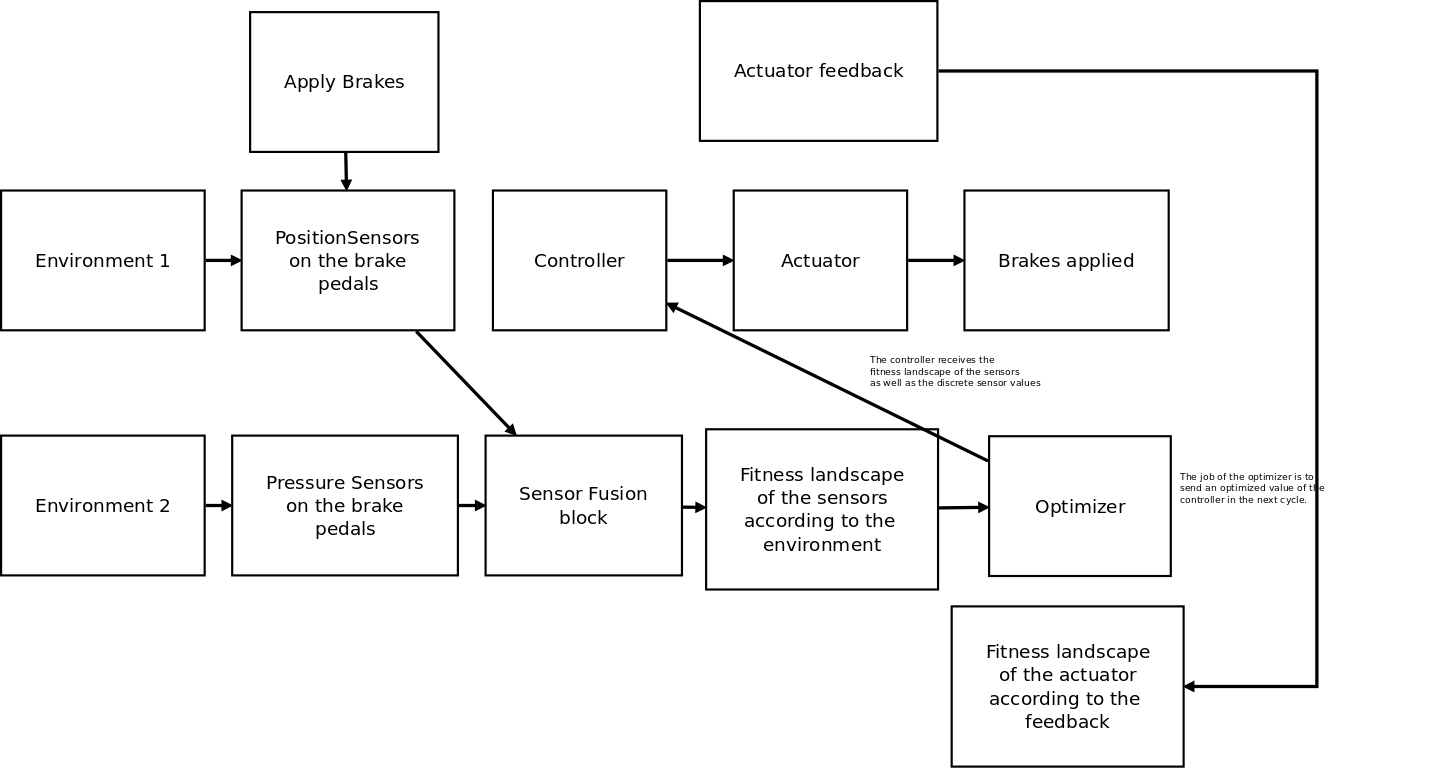
\includegraphics[width=1.0\textwidth]{images/second.png}
\caption{Overview}
\label{fig:Overview}
\end{center}
\end{figure}

%\include{parts/Grundlagen}


%\include{parts/Ausblick}



%\include{parts/Danksagung} % Danksagung



%%%%%%%%% Anhang, Literaturverzeichnis %%%%%%%%%%%%%
%\include{parts/anhang} % Anhang
%\include{parts/Software} % Software

%------------- Altes Abb. Verzeichnis in Gruppen
\phantomsection
\addcontentsline{toc}{chapter}{List of Figures}
\listoffigures % Bilderverzeichnis

\clearpage
\phantomsection
\addcontentsline{toc}{chapter}{List of Tables}
\listoftables % Tabellenverzeichnis}
\clearpage


\phantomsection
\addcontentsline{toc}{chapter}{List of Listings}
\lstlistoflistings
%\renewcommand{\lstlistlistingname}{List of Listings}
%\renewcommand{\lstlistingname}{List of Listings}
%\lstlistoflistings
\clearpage

%%\begingroup
%%\phantomsection
%%\addcontentsline{toc}{chapter}{\listfigurename}
%%\renewcommand*{\addvspace}[1]{}
%%\listoffigures
%%\cleardoublepage
%%\phantomsection
%%\addcontentsline{toc}{chapter}{\listtablename}
%%\listoftables
%%\endgroup

%------------- Altes Abb. Verzeichnis ohne Gruppen
%%\begingroup
%%\phantomsection
%%\addcontentsline{toc}{chapter}{\listfigurename}
%%\renewcommand*{\addvspace}[1]{}
%%\listoffigures
%%\cleardoublepage
%%\phantomsection
%%\addcontentsline{toc}{chapter}{\listtablename}
%%\listoftables
%%\endgroup

\phantomsection
\addcontentsline{toc}{chapter}{Bibliography}
\bibliography{Quellen}
\bibliographystyle{alpha}


\end{document}
% ENDE
